\documentclass[letter]{article}

%% Language and font encodings
\usepackage[english]{babel}
\usepackage[utf8x]{inputenc}
\usepackage[T1]{fontenc}
\usepackage{enumitem}
\usepackage{fancyhdr}
\pagestyle{fancy}

%% Useful packages
\usepackage{amsmath, amsthm, amssymb}
\usepackage{graphicx}
\newtheoremstyle{case}{}{}{}{}{}{:}{ }{}
\theoremstyle{case}
\newtheorem{case}{}


\title{HW Template}
\author{Nicholas Silva Tee}
\lhead{Homework Template}



\begin{document}

\subsection*{Problem 1}
\textbf{a. } 3 x 2 x 2 x 3 x 4 = 144 --> $2^{144}$ nanoseconds\\
\textbf{b. } 4 x 3 x 3 x 4 x 5 = 720 nanoseconds\\
\textbf{c. } $(2^3-1)(2^2-1)(2^2-1)(2^3-1)(2^4-1)$ \\
7 x 3 x 3 x 7 x 15 = 6615 nanoseconds

\subsection*{Problem 2}
Point: [2, 2, 3, '+']    \textbf{a)} 0.743    \textbf{b)} 0     \textbf{c)} 0.257     \textbf{d)} 0.066 \\
Point: [3, 3, 2, '+']    \textbf{a)} 0.928    \textbf{b)} 0     \textbf{c)} 0.072     \textbf{d)} 0.005 \\
Point: [1, 2, 3, '+']    \textbf{a)} 0.186    \textbf{b)} 0     \textbf{c)} 0.814     \textbf{d)} 0.663 \\
Point: [1, 4, 1, '+']    \textbf{a)} -0.557    \textbf{b)} 1     \textbf{c)} 1.557     \textbf{d)} 2.425 \\
Point: [4, 4, 4, '+']    \textbf{a)} 3.343    \textbf{b)} 0     \textbf{c)} 0     \textbf{d)} 0 \\
Point: [2, 2, 2, '+']    \textbf{a)} 0.0    \textbf{b)} 1     \textbf{c)} 1.0     \textbf{d)} 1.0 \\
Point: [3, 3, 1, '-']    \textbf{a)} -0.186    \textbf{b)} 1     \textbf{c)} 1.186     \textbf{d)} 1.406 \\
Point: [1, 1, 1, '-']    \textbf{a)} 1.671    \textbf{b)} 0     \textbf{c)} 0     \textbf{d)} 0 \\
Point: [3, 3, 2, '-']    \textbf{a)} -0.928    \textbf{b)} 1     \textbf{c)} 1.928     \textbf{d)} 3.719 \\
Point: [0, 4, 2, '-']    \textbf{a)} 0.371    \textbf{b)} 0     \textbf{c)} 0.629     \textbf{d)} 0.395 \\
Point: [4, 0, 0, '-']    \textbf{a)} 1.114    \textbf{b)} 0     \textbf{c)} 0     \textbf{d)} 0 \\
Point: [0, 0, 3, '-']    \textbf{a)} 1.114    \textbf{b)} 0     \textbf{c)} 0     \textbf{d)} 0 \\
\newpage
\subsection*{Problem 3}
\begin{table}[!h]
\begin{tabular}{lllll}
1 & 0.1 & 0.114 & 0.114 & 0.14 \\
2 & 0.2 & 0.2   & 0.2   & 0.2  \\
3 & 0.3 & 0.286 & 0.286 & 0.26 \\
4 & 0   & 0.029 & 0.029 & 0.08 \\
5 & 0.4 & 0.371 & 0.371 & 0.32
\end{tabular}
\end{table}
\begin{figure}[h!]
	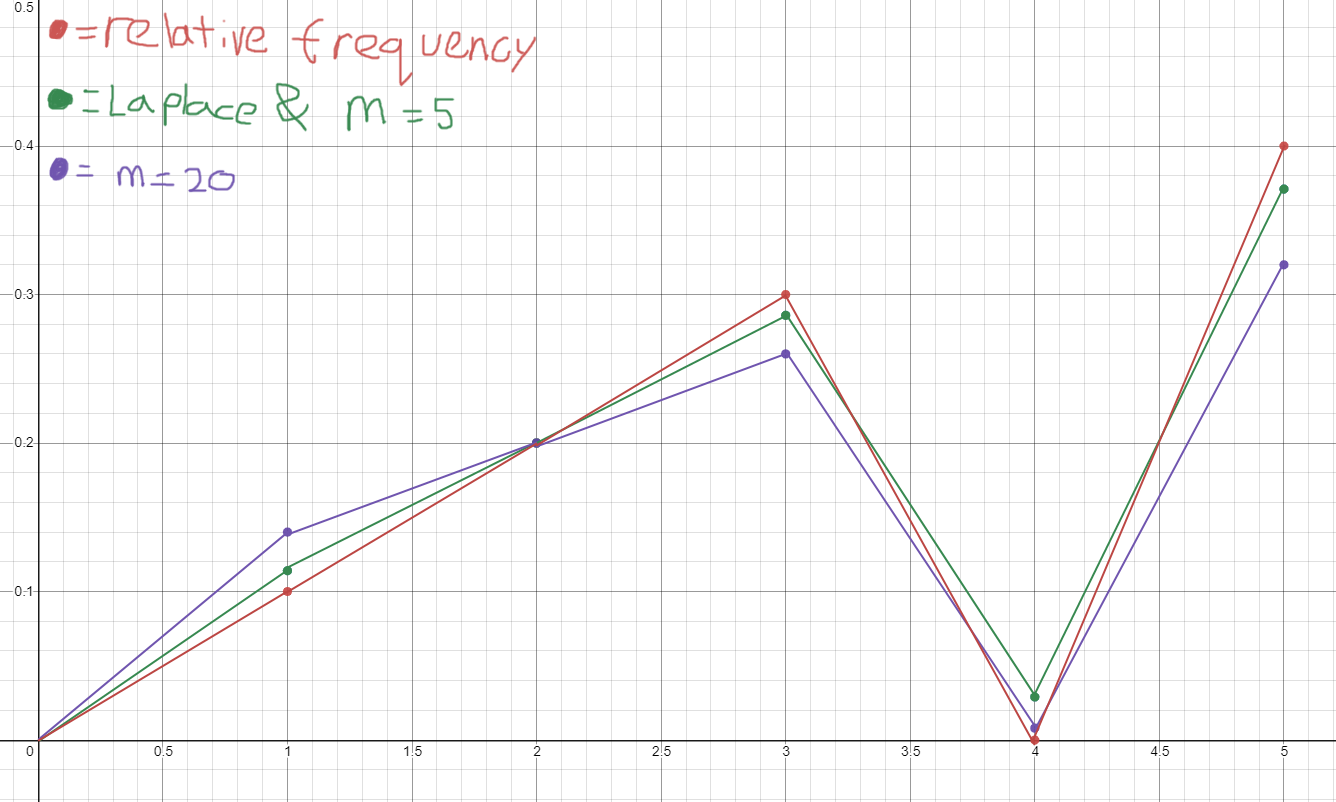
\includegraphics[scale=0.4]{all.png}
\end{figure} 
As the number of the pseudo counts increases, the probabilities of the 4 classes grows closer to the overall average which would have been 1/5
\newpage
\subsection*{Problem 4}
\textbf{a. } 4 x 4 x 3 x 3 = 144 --> $2^{144}$ conjunctive hypotheses \\
\textbf{b. } (Budget=[Low,High], Genre=Drama, Director=Great) \\
\textbf{c. } (Genre = drama) \\
\textbf{d. } (Budget=Low, Genre=Drama, Famous Actors=No, Director=Great)
\subsection*{Problem 5}
\begin{table}[!h]
\begin{tabular}{|l|l|l|l|l|}
\hline
                    & p   & weight & impurity & Feature impurity \\ \hline
Budget = low        & 1/3 & 6/16   & 0.918    &                  \\ \cline{1-4}
Budget = medium     & 3/5 & 5/16   & 0.971    & 0.873            \\ \cline{1-4}
Budget = high       & 4/5 & 5/16   & 0.722    &                  \\ \hline
Genre = Documentary & 2/5 & 5/16   & 0.971    &                  \\ \cline{1-4}
Genre = Drama       & 5/6 & 3/8    & 0.65     & 0.85             \\ \cline{1-4}
Genre = Comedy      & 2/5 & 5/16   & 0.971    &                  \\ \hline
FamousActor = Yes   & 5/8 & 1/2    & 0.954    & 0.977            \\ \cline{1-4}
FamourActor = No    & 1/2 & 1/2    & 1        &                  \\ \hline
Director = Great    & 5/7 & 7/16   & 0.863    & 0.935            \\ \cline{1-4}
Director = Unknown  & 4/9 & 9/16   & 0.991    &                  \\ \hline
\end{tabular}
\end{table}
This means that our root node will be the "Genre" feature \\
\begin{table}[!h]
\begin{tabular}{|l|l|l|l|l|}
\hline
\multicolumn{5}{|c|}{Genre=Documentary}                         \\ \hline
                   & p   & weight & impurity & Feature impurity \\ \hline
Budget = low       & 0   & 2/5    & 0        &                  \\ \cline{1-4}
Budget = medium    & 2/3 & 3/5    & 0.918    & 0.55             \\ \cline{1-4}
Budget = high      & 0   & 0      & N/A      &                  \\ \hline
FamousActor = Yes  & 1/3 & 3/5    & 0.918    & 0.95             \\ \cline{1-4}
FamourActor = No   & 1/2 & 2/5    & 1        &                  \\ \hline
Director = Great   & 0   & 1/5    & 0        & 0.8              \\ \cline{1-4}
Director = Unknown & 1/2 & 4/5    & 1        &                  \\ \hline
\end{tabular}
\end{table} \\
Next node will be Budget
\newpage
\begin{table}[!h]
\begin{tabular}{|l|l|l|l|l|}
\hline
\multicolumn{5}{|c|}{Genre=Comedy}                              \\ \hline
                   & p   & weight & impurity & Feature impurity \\ \hline
Budget = low       & 1/2 & 2/5    & 1        &                  \\ \cline{1-4}
Budget = medium    & 0   & 1/5    & 0        & 0.8              \\ \cline{1-4}
Budget = high      & 1/2 & 2/5    & 1        &                  \\ \hline
FamousActor = Yes  & 1   & 1/5    & 0        & 0.649            \\ \cline{1-4}
FamourActor = No   & 1/4 & 4/5    & 0.811    &                  \\ \hline
Director = Great   & 2/3 & 3/5    & 0.918    & 0.589            \\ \cline{1-4}
Director = Unknown & 0   & 2/5    & 0        &                  \\ \hline
\end{tabular}
\end{table} 
Next node will be director \\
\begin{table}[!h]
\begin{tabular}{|l|l|l|l|l|}
\hline
\multicolumn{5}{|c|}{Genre=Drama}                              \\ \hline
                   & p   & weight & impurity & Feature impurity \\ \hline
Budget = low       & 1/2 & 2/6    & 1        &                  \\ \cline{1-4}
Budget = medium    & 1   & 1/6    & 0        & 0.333            \\ \cline{1-4}
Budget = high      & 1   & 3/6    & 0        &                  \\ \hline
FamousActor = Yes  & 3/4 & 4/6    & 0.811    & 0.541            \\ \cline{1-4}
FamourActor = No   & 1   & 2/6    & 0        &                  \\ \hline
Director = Great   & 1   & 1/2    & 0        & 0.459            \\ \cline{1-4}
Director = Unknown & 2/3 & 1/2    & 0.918    &                  \\ \hline
\end{tabular}
\end{table} \\
Next node will be budget \\
\newpage
\begin{table}[!h]
\begin{tabular}{|l|l|l|l|l|}
\hline
\multicolumn{5}{|c|}{Genre=Documentary and Budget=Low}             \\ \hline
                   & p & weight & impurity & Feature impurity \\ \hline
FamousActor = Yes  & 0 & 1      & 0        & 0                \\ \cline{1-4}
FamourActor = No   & 0 & 0      & N/A        &                  \\ \hline
Director = Great   & 0 & 1/2    & 0        & 0                \\ \cline{1-4}
Director = Unknown & 0 & 1/2    & 0        &                  \\ \hline
\end{tabular}
\end{table}
next node is FamousActor \\
\begin{table}[!h]
\begin{tabular}{|l|l|l|l|l|}
\hline
\multicolumn{5}{|c|}{Genre=Documentary and Budget=Medium}               \\ \hline
                   & p   & weight & impurity & Feature impurity \\ \hline
FamousActor = Yes  & 1   & 1/3    & 0        & 0.667            \\ \cline{1-4}
FamourActor = No   & 1/2 & 2/3    & 1        &                  \\ \hline
Director = Great   & 0   & 0      & N/A      & 0.918            \\ \cline{1-4}
Director = Unknown & 2/3 & 1      & 0.918    &                  \\ \hline
\end{tabular}
\end{table} \\
next node is FamousActor \\
\begin{table}[!h]
\begin{tabular}{|l|l|l|l|l|}
\hline
\multicolumn{5}{|c|}{Genre=Comedy and Director=Great}          \\ \hline
                & p & weight & impurity & Feature impurity \\ \hline
Budget = Low    & 1 & 1/3    & 0        &                  \\ \cline{1-4}
Budget = Medium & 0 & 1/3    & N/A      & 0                \\ \cline{1-4}
Budget = High   & 1 & 1/3    & 0        &                  \\ \hline
\end{tabular}
\end{table} \\
Since budget's impurity value is 0 then we default to that as the next node. Same case for Director=unknown \\

\begin{table}[!h]
\begin{tabular}{|l|l|l|l|l|}
\hline
\multicolumn{5}{|c|}{Genre=Drama and Budget=Low}              \\ \hline
                   & p & weight & impurity & Feature impurity \\ \hline
FamousActors = Yes & 0 & 1/2    & N/A      & 0.5              \\ \cline{1-4}
FamousActors = No  & 1 & 1/2    & 1        &                  \\ \hline
Director = Great   & 1 & 1/2    & 1        &                  \\ \cline{1-4}
Director = Unknown & 0 & 1/2    & N/A      & 0.5              \\ \hline
\end{tabular}
\end{table} 
Next node is FamousActors \\
\begin{figure}[h!]
	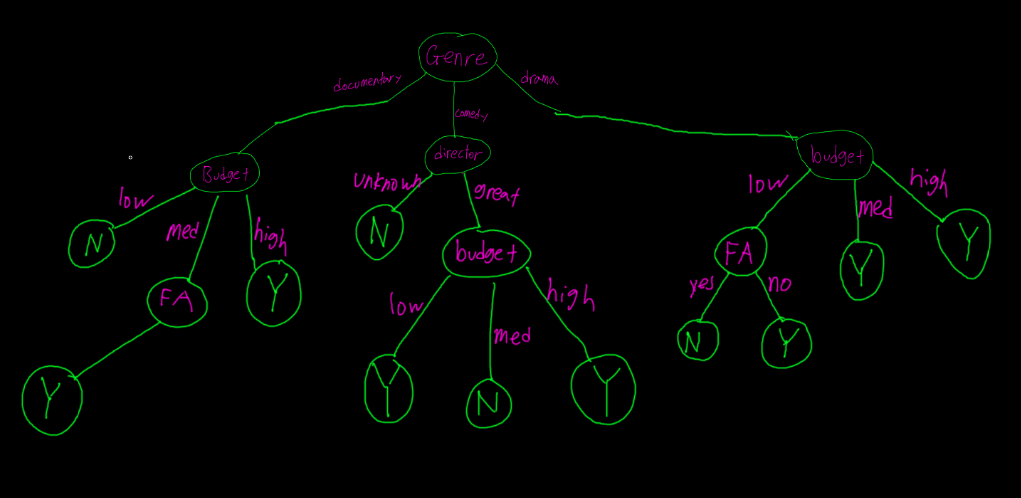
\includegraphics[scale=0.4]{part2.png}
\end{figure}
\newpage
\textbf{Training Data} \\
\textbf{Labelled Yes: } 1 2 3 4 5 6 7 9 10 111 12 13 14 15 16 \\
\textbf{Labelled No: } 8 \\
\textbf{Error Rate: } 15/16 \\

\textbf{Test Data 1} \\
\textbf{Labelled Yes: } 5 6 9 11 12 13 14 15 17 18 19\\
\textbf{Labelled No: } 1 2 3 4 7 8 10 16 20 \\
\textbf{Error Rate: } 9/20\\

\textbf{Test Data 2} \\
\textbf{Labelled Yes: } 1 3 4 5 6 8 9 11 12 14 16 17 19 20 \\
\textbf{Labelled No: } 2 7 10 13 15 18 \\
\textbf{Error Rate: } 6/20\\

\textbf{Test Data 3} \\
\textbf{Labelled Yes: } 1 3 4 5 6 8 9 11 12 13 14 15 16\\
\textbf{Labelled No: } 2 7 10 13 15 \\
\textbf{Error Rate: } 5/20\\
\newpage
\subsection*{Problem 6}
For my program I took the following steps \\
\textbf{1.} Sort the training data into 3 seperate arrays, 1 per class \\
\textbf{2.} Find the centroids of each of the classes \\
\textbf{3.} Create a normalized vector between two centroids and find the "d" value by inputting a midpoint\\
\textbf{4.} Once the equations are created I check for each point for what side of the plane it is on.\\
\textbf{5.} Checking with the 01 discriminant function if the value is positive then it chooses class 0 and compares with the 20 discriminant function to choose between class 2 and 0.\\
\textbf{6.} Step 5 is repeated for each point.\\

\textbf{Performance} \\
\textbf{Test 1 accuracy: } 9 Errors out of 75 points\\
\textbf{Test 2 accuracy: } 33 Errors out of 300 points\\

\textbf{CodaLab Performance} \\
\textbf{Accuracy:}  0.93\\
\textbf{Precision:} 0.89 \\
\textbf{F measure:} 0.89 \\
\textbf{Recall:} 0.89 \\
\textbf{F1 Score:} 0.89\\
\end{document}










